\chapter{Onde piane TEM tra due materiali} 
\begin{figure}[h]
    \centering
    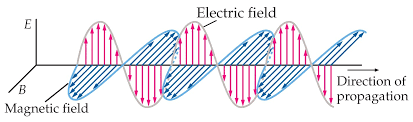
\includegraphics{TEM plane waves.png}
    
\end{figure}    

\newpage

\section{Riflessione e trasmissione delle onde piane con incidenza normale (TEM)}

\footnote{FCE - Pag 311 | 8.1.1 Interfaccia tra mezzi senza perdite \\ 
FAE - Pag 339 | 8.1.1 Boundary between lossless media} 

Per onde TEM (Transverse Electro-Magnetic Waves) si intendono onde in cui campi 
elettrico e magnetico hanno direzione ortogonale rispetto a quella del vettore di propagazione. 

\begin{figure}[h]
    \centering
    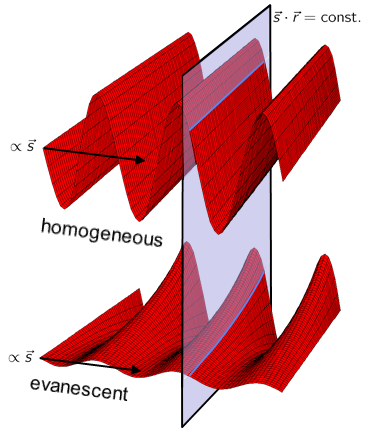
\includegraphics{plane_waves_hom_evan.png}    
\end{figure}    
\footnote{\url{https://www.pvlighthouse.com.au/it/cms/lectures/altermatt/optics/planar-transversal-electromagnetic-waves}} 


Consideriamo questo piano: 

\begin{figure}[h]
    \centering
    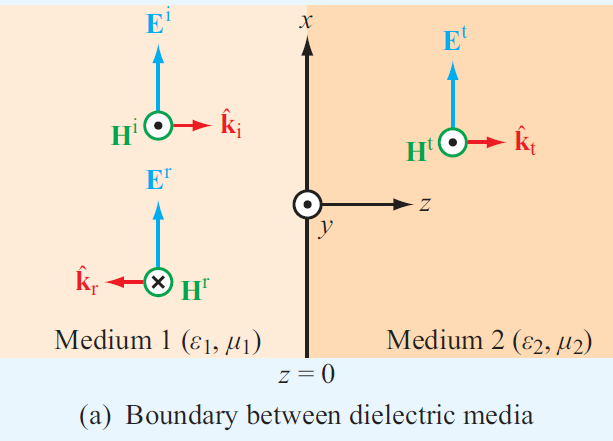
\includegraphics[scale = 0.6]{TEM EM waves.PNG}    
\end{figure}    
\footnote{FAE - pag 340}

in cui il tondino con il punto indica che l'asse esce dal foglio. \\

Possiamo rappresentare, dal punto di vista grafico, anche in questa maniera: \\ \\ 

\begin{figure}[h]
    \centering
    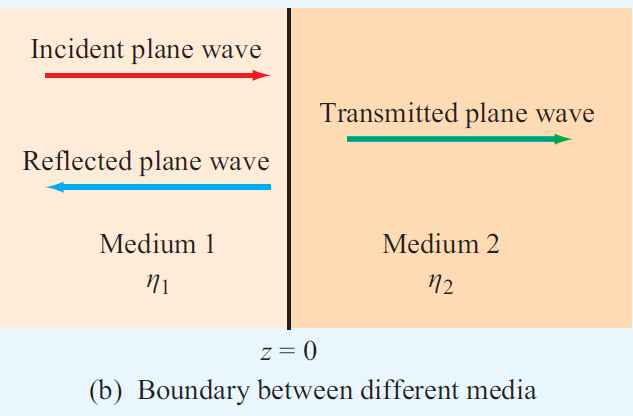
\includegraphics[scale = 0.6]{EM between two mediums.PNG}    
\end{figure}

\footnote{FAE - pag 339}


Esplicitiamo le equazioni delle onde piane: \\ \\ 

\textbf{Onda incidente:} 
{\Large \begin{equation}
    \begin{cases}
        \vec{E^{i}}(z) = \hat{x} E_o ^{i} e^{-\jmath \kappa_1 z} \\ 
        \vec{H^{i}}(z) = \hat{y} \frac{E_o ^{i}}{\eta_1} e^{-\jmath \kappa_1 z}  
    \end{cases}
\end{equation}}


\textbf{Onda riflessa:} 
{\Large \begin{equation}
    \begin{cases}
        \vec{E^{r}}(z) = \hat{x} E_o ^{r} e^{\jmath \kappa_1 z} \\ 
        \vec{H^{r}}(z) = -\hat{y} \frac{E_o ^{r}}{\eta_1} e^{\jmath \kappa_1 z}  
    \end{cases}
\end{equation}}

\textbf{Onda trasmessa:} 
{\Large \begin{equation}
    \begin{cases}
        \vec{E^{t}}(z) = \hat{x} E_o ^{t} e^{-\jmath \kappa_2 z} \\ 
        \vec{H^{t}}(z) = \hat{y} \frac{E_o ^{t}}{\eta_2} e^{-\jmath \kappa_2 z}  
    \end{cases}
\end{equation}}

dove: 

{\Large \begin{equation}
    \begin{cases}
        \kappa_1 = \omega \sqrt{\mu_1 \varepsilon_1} \\ 
        \kappa_2 = \omega \sqrt{\mu_2 \varepsilon_2} \\ 
        \eta_1 = \sqrt{\frac{\mu_1}{\varepsilon_1}} \\ 
        \eta_2 = \sqrt{\frac{\mu_2}{\varepsilon_2}} \\ 
    \end{cases}
\end{equation}}

$E_o ^{i}$, $E_o ^{r}$,  $E_o ^{t}$ sono le ampiezze delle onde, rispettivamente, dell'onda incidente, riflessa e trasmessa. \\ 

I numeri dei coefficienti (1 e 2) indicano in quale piano si trovano le onde. \\ \\ 

Dal capitolo 4 sulla continuità dei campi, sappiamo che il componente tangente di $\vec{E}$ è sempre continuo in un'interfaccia tra due mezzi adiacenti. \\ 
Inoltre, in assenza di corrente sull'interfaccia, anche il componente tangenziale di $\vec{H}$ è continuo tra due mezzi adiacenti. \\ \\ 

Quindi nel mezzo 1, l'onda sarà: \\ 

{\Large \begin{equation}
    \begin{cases}
        \vec{E_1 }(z) = \vec{E^{i}} (z) + \vec{E^{r} }(z) = \hat{x} (E_o ^{i} e^{-\jmath \kappa_1 z} + E_o ^{r} e^{\jmath \kappa_1 z} ) \\ 
        \vec{H_1} (z) = \vec{H^{i}} (z) + \vec{H^{r}} (z) = \hat{y} \frac{1}{\eta_1} (E_o ^{i} e^{-\jmath \kappa_1 z} + E_o ^{r} e^{\jmath \kappa_1 z} )    
    \end{cases}
\end{equation}}

Per adesso, nel mezzo 2 è solo presente l'onda trasmessa, quindi: 

{\Large \begin{equation}
    \begin{cases}
        \vec{E_2} (z) = \vec{E^{t}} (z) = \hat{x} E_o ^{t} e^{-\jmath \kappa_2 z} \\ 
        \vec{H_2} (z) = \vec{H^{t}} (z) = \hat{y} \frac{E_o ^{t}}{\eta_2} e^{-\jmath \kappa_2 z}    
    \end{cases}
\end{equation}}

Ponendoci all'interfaccia $z = 0$, i componenti tangenziali dei campi elettrico e magnetico sono continui. \\ 

In formule: 

{\Large \begin{equation}
    \begin{cases}
        \vec{E_1} (z = 0) = \vec{E_2} (z= 0) \Rightarrow E_o ^{i} + E_o ^{r} = E_o ^{t} \\ 
        \vec{H_1} (z = 0) = \vec{H_2} (z= 0) \Rightarrow \frac{E_o ^{i}}{\eta_1} - \frac{E_o ^{r}}{\eta_1} = \frac{E_o ^{t}}{\eta_2} 
    \end{cases}
\end{equation}}

Risolvendo il sistema per ricavare $E_o ^{r}$ in funzione di $E_o ^{i}$ (quindi poniamo $E_o ^{i}$ come variabile indipipenente), 
avremo che: 

{\Large \begin{equation}
    \begin{split}
        E_o ^{r} 
        &= \frac{\eta_2 - \eta_1}{\eta_2 + \eta_1} E_o ^{i} 
        \\
        &= \Gamma E_o ^{i}   
    \end{split}
\end{equation}}

\begin{tcolorbox}
    $\Gamma$ si legge gamma 
\end{tcolorbox}

Risolvendo il sistema per ricavare $E_o ^{t}$ in funzione di $E_o ^{i}$, avremo che: 

{\Large \begin{equation}
    \begin{split}
        E_o ^{t} 
        &= \frac{2 \eta_2 }{\eta_2 + \eta_1} E_o ^{i} 
        \\
        &=  \tau E_o ^{i}   
    \end{split}
\end{equation}}

dove: 

{\Large \begin{equation}
    \Gamma = \frac{E_o ^{r}}{E_o ^{i}} = \frac{\eta_2 - \eta_1}{\eta_2 + \eta_1}
\end{equation}}

$\Gamma$ prende il nome di coefficiente di riflessione. 

{\Large \begin{equation}
    \tau = \frac{E_o ^{t}}{E_o ^{i}} = \frac{2 \eta_2}{\eta_2 + \eta_1} 
\end{equation}}

$\tau$ prende il nome di coefficiente di trasmissione. \\ 

Se $\eta_1$ e $\eta_2$ sono reali, anche $\Gamma$ e $\tau$ lo sono. \\ \\  

$\tau$ si può esprimere come: 

{\Large \begin{equation}
    \tau = 1 + \Gamma    
\end{equation}}

Si può esprimere $\eta_1$ e $\eta_2$ come: 

{\Large \begin{equation}
    \begin{cases}
        \eta_1 = \frac{\eta_o}{\sqrt{\varepsilon_{r1}}} \\ 
        \eta_2 = \frac{\eta_o}{\sqrt{\varepsilon_{r2}}} 
    \end{cases}
\end{equation}}

dove: 

{\Large \begin{equation}
    \eta_o = \sqrt{\frac{\mu_o}{\varepsilon_o}} \approx 377 [\Omega] 
\end{equation}}

$\eta_o$ prende il nome di impedenza intrinsica nello spazio libero. \\ \\ 

$\Gamma$ si può scrivere nei materiali non magnetici anche come: \\

{\Large \begin{equation}
    \Gamma = \frac{\sqrt{\varepsilon_{r1}} - \sqrt{\varepsilon_{r2}}}{ \sqrt{\varepsilon_{r1}} + \sqrt{\varepsilon_{r2}}}
\end{equation}}

\newpage 

\section{Flusso di potenza nei mezzi senza perdite} 

\footnote{FCE - pag 315 | 8.1.3 Flusso di potenza nei mezzi senza perdite \\ 
FAE - pag 341 | 8.1.1 Power Flow in Lossless media}

Utilizzando il teorema di Poynting, la densità media netta che flusice nel mezzo 1 è: 

{\Large \begin{equation}
    \begin{split}
        \vec{S_{av_1}} &= \frac{1}{2} \Re [\vec{E_1}(z) \times \vec{H_1} ^ {*} (z) ] 
        \\
        &= \frac{1}{2} \Re [\hat{x} E_o ^{i} (e^{-\jmath \kappa_1 z} + \Gamma e^{\jmath \kappa_1 z}) \times  \hat{y} \frac{E_o ^{i^*}}{\eta_1} (e^{\jmath \kappa_1 z} - \Gamma e^{-\jmath \kappa_1 z})]\\ 
        &= \hat{z} \frac{\left|E_o ^{i}\right| ^{2}}{2 \eta_1} (1 - \left|\Gamma\right| ^{2})    
    \end{split}
\end{equation}} 

$\vec{S_{av_1}}$ lo si può esprimere anche come: 

{\Large \begin{equation}
    \vec{S_{av_1}} = \vec{S_{av} ^{i}} + \vec{S_{av} ^{r}}    
\end{equation}} 

dove: 

{\Large \begin{equation}
    \begin{cases}
        \vec{S_{av} ^{i}} = \hat{z} \frac{\left|E_o ^{i}\right|}{2 \eta_1} \\ 
        \vec{S_{av} ^{r}} = - \hat{z}  \left|\Gamma\right|^{2} \frac{\left|E_o ^{i}\right|}{2 \eta_1} = - \left|\Gamma\right|^{2} \vec{S_{av} ^{i}}\\ 
    \end{cases}
\end{equation}}

$\vec{S_{av} ^{i}}$ è la densità di energia media dell'onda incidente nel mezzo 1, 
mentre $\vec{S_{av} ^{r}}$ è la densità di energia media dell'onda riflessa nel mezzo 1. \\ \\ 

La densità di potenza media nel mezzo 2 è: 

{\Large \begin{equation}
    \begin{split}
    \vec{S_{av_2}} &= \frac{1}{2} \Re [\vec{E_2}(z) \times \vec{H_2} ^ {*} (z) ] \\
    &= \frac{1}{2} \Re [\hat{x} \tau E_o ^{i} e^{-\jmath \kappa_2 z} \times  \hat{y} \tau^{*} \frac{E_o ^{i^*}}{\eta_2} e^{\jmath \kappa_2 z}] \\ 
    &= \hat{z} \left|\tau\right| ^{2} \frac{\left|E_o ^{i}\right| ^{2}}{2 \eta_2}
    \end{split}
\end{equation}}

Nei mezzi senza perdite: 
{\Large \begin{equation}
    \frac{\tau ^{2}}{\eta_2} = \frac{1 - \Gamma ^{2}}{\eta_1}
\end{equation}} 

da cui: 

{\Large \begin{equation}
    \vec{S_{av_1}} = \vec{S_{av_2}} 
\end{equation}}

\newpage


\section{Leggi di Snell} 

\footnote{FCE - pag 322 | 8.2 Legge di Snell \\ 
FAE - pag 349 | 8.2 Snell's Laws} 

\begin{figure}[h]
    \centering
    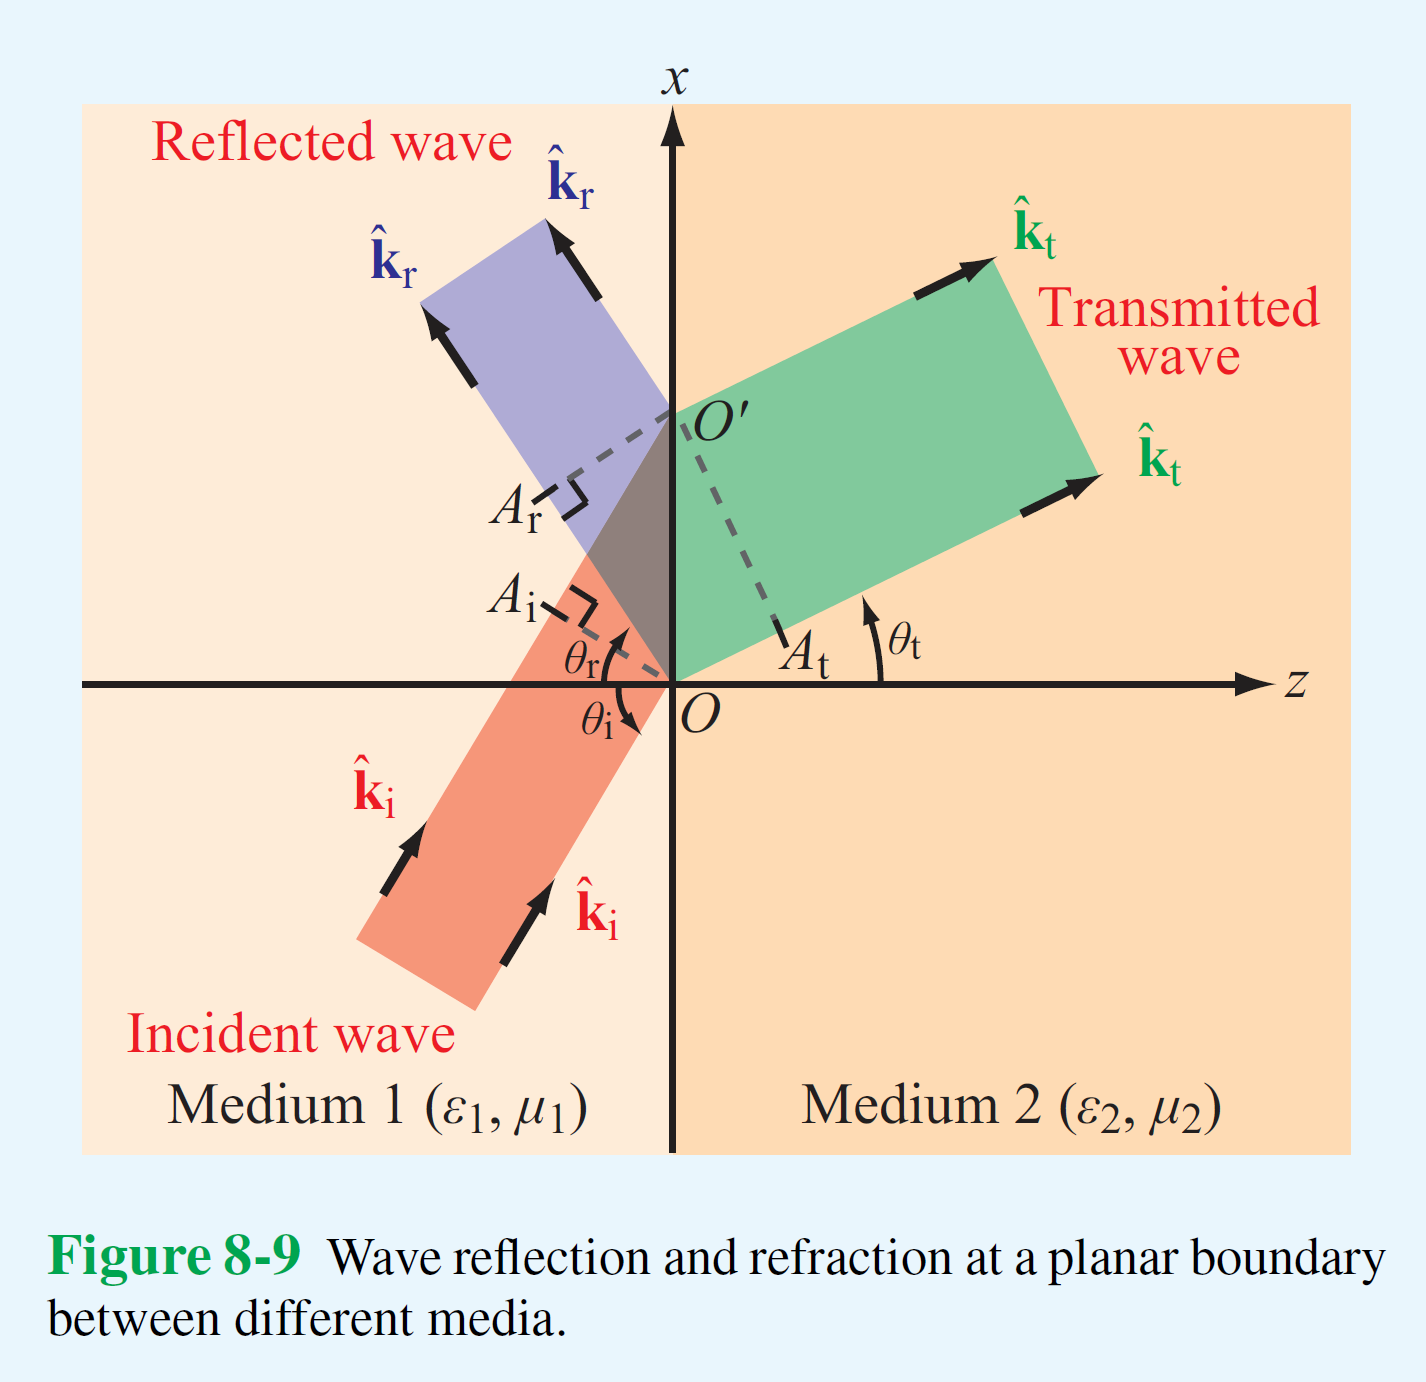
\includegraphics[scale = 0.8]{Wave reflectaion in a boundary.PNG}
    
\end{figure} 

Considerando un'interfaccia a $z=0$ per due mezzi diversi, mezzo 1 con $\varepsilon_1$, $\mu_1$ e 
mezzo 2 con $\varepsilon_2$, $\mu_2$ e: \\ 

$\theta_i$ angolo di incidenza \\ 
$\theta_r$ angolo di riflessione \\ 
$\theta_t$ angolo di trasmissione (o rifrazione) \\ \\ 

Indicando con $u_{p_1}$ e $u_{p_2}$ le velocità dell'onda nei mezzi 1 e 2: 

{\Large \begin{equation}
    \begin{cases}
        u_{p_1} = \frac{1}{\sqrt{\mu_1 \varepsilon_1}}\\ 
        u_{p_2} = \frac{1}{\sqrt{\mu_2 \varepsilon_2}} 
    \end{cases}
\end{equation}} 

Possiamo esprimere le leggi di Snell: 

{\Large \begin{equation}
    \begin{cases}
        \theta_i = \theta_r \\ 
        \frac{\sin(\theta_t)}{\sin(\theta_i)} = \frac{u_{p_2}}{u_{p_1}} = 
        \sqrt{\frac{\mu_1 \varepsilon_1}{\mu_2 \varepsilon_2}} = \frac{n_1}{n_2}   
    \end{cases}
\end{equation}}

La prima equazione prende il nome di Legge di Snell della riflessione, 
la seconda equazione prende il nome di Legge di Snell della rifrazione. \\ \\ 

Per materiali non magnetici, dove $\mu_1 = \mu_2$, la legge di Snell della rifrazione diventa: 

{\Large \begin{equation}
    \frac{\sin(\theta_t)}{\sin(\theta_i)} = \frac{n_1}{n_2} = 
    \sqrt{\frac{\varepsilon_{r_1}}{\varepsilon_{r_2}}} = \frac{\eta_1}{\eta_2}
\end{equation}}

dove: 

{\Large \begin{equation}
    n = \sqrt{\varepsilon_r}
\end{equation}}

Ricordando che l'inidice di rifrazione come: 

{\Large \begin{equation}
    n = \frac{c}{u_p} = \sqrt{\frac{\mu \varepsilon}{\mu_o \varepsilon_o}} = \sqrt{\mu_r \varepsilon_r}
\end{equation}}


Si dice che un materiale è più denso se $n_1 > n_2$. \\ \\ 

Utilizzando le leggi di Snell possiamo dire che se: 

{\Large \begin{equation}
    \begin{cases}
        \theta_i = 0 \Rightarrow \theta_t = 0 \\ 
        \theta_t < \theta_i \Rightarrow n_2 > n_1 \\ 
        \theta_t > \theta_i \Rightarrow n_2 < n_1 \\ 
        \theta_t = \frac{\pi}{2} = E_o ^{t} = 0
    \end{cases}
\end{equation}}

Nell'ultimo caso $\theta_t$ viene chiamato $\theta_c$ (angolo critico) 
perchè è quell'angolo per cui l'onda non viene trasmessa nell'altro mezzo e viene completamente riflessa. \\ 

Per le onde TEM: 

{\Large \begin{equation}
    \sin(\theta_c) = \sqrt{\frac{\varepsilon_{r_2}}{\varepsilon_{r_1}}}
\end{equation}}

Se $\theta_i > \theta_c$ allora l'onda viene completamente riflessa. \\ \\

\begin{figure}[h]
    \centering
    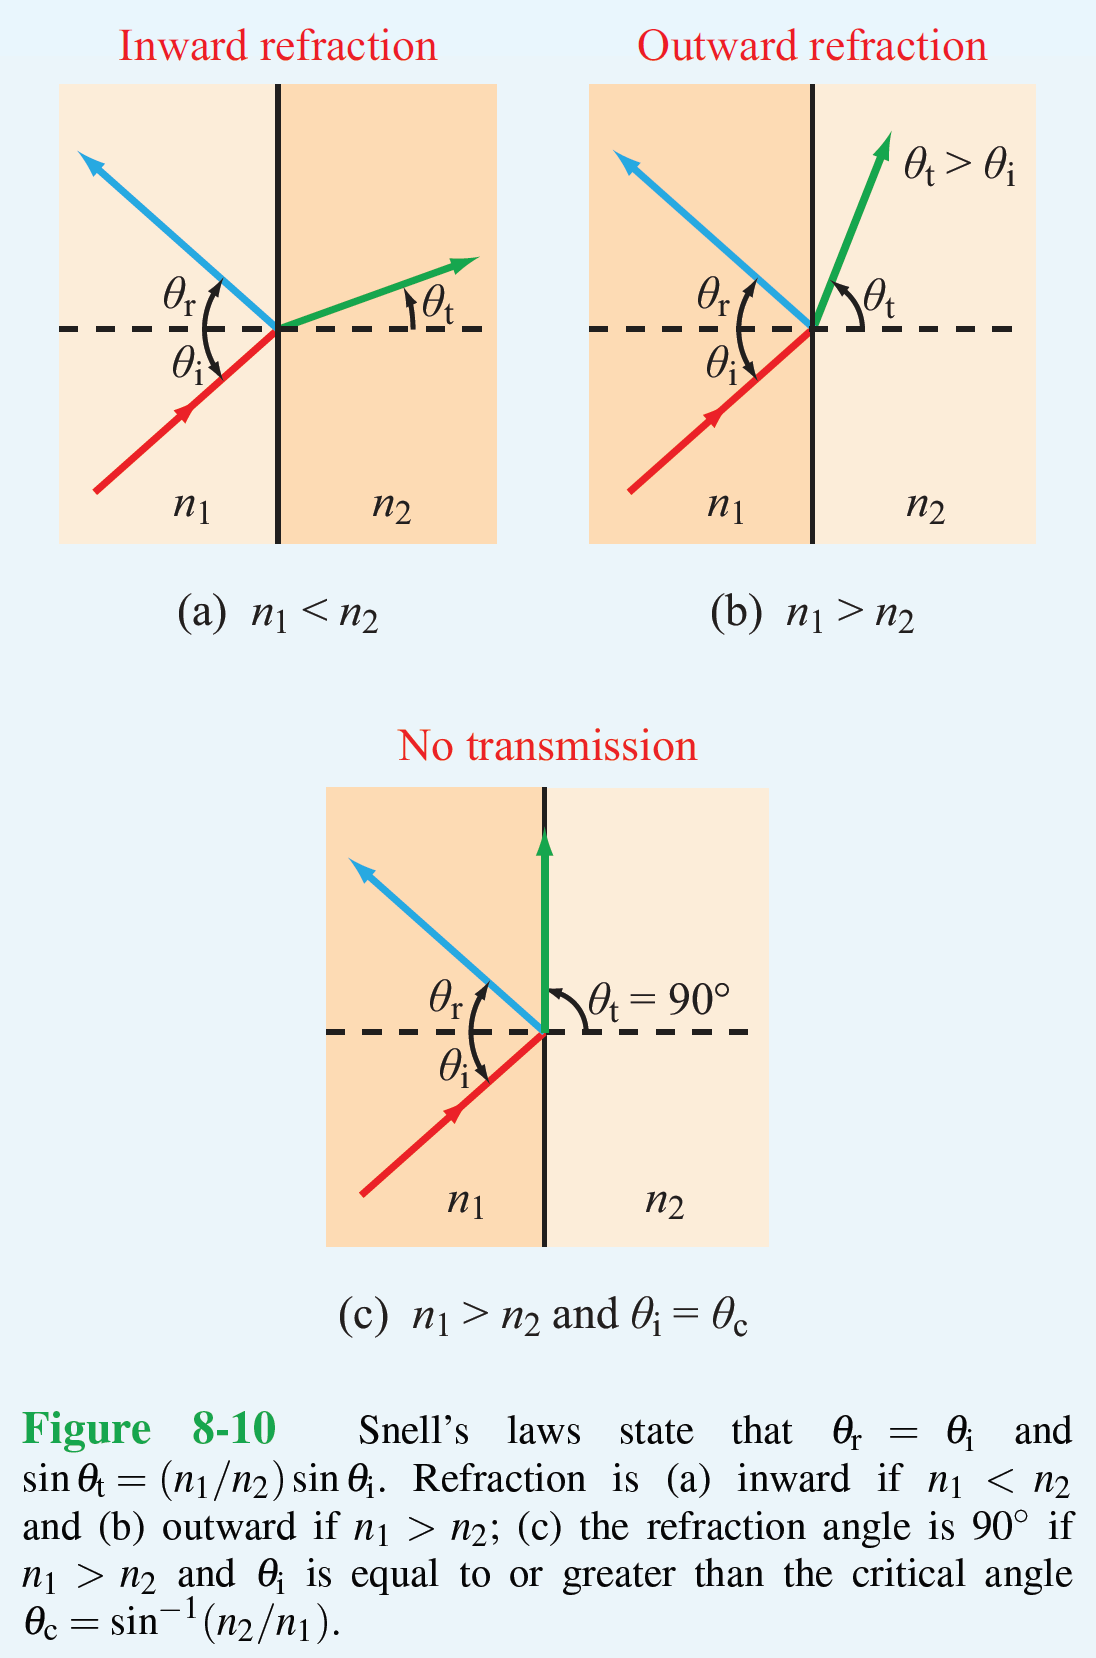
\includegraphics{Snell's laws and different angles.PNG}
    
\end{figure} 

\footnote{FAE - pag 350} 

\newpage 
